\documentclass[10pt,a4paper]{article}
\usepackage[margin=0.7in]{geometry}
\usepackage{multicol}
\usepackage{amsmath}
\usepackage{tikz}
\usepackage{enumitem}
\usepackage{titlesec}
\usepackage{booktabs}
\usepackage{fontspec}

% Compact formatting
\setlength{\columnsep}{0.7cm}
\setlength{\parindent}{0pt}
\setlength{\parskip}{0.12cm}
\titlespacing{\section}{0pt}{0.4cm}{0.15cm}
\titlespacing{\subsection}{0pt}{0.25cm}{0.08cm}
\titlespacing{\subsubsection}{0pt}{0.2cm}{0.05cm}

% Custom section style
\titleformat{\section}{\large\bfseries}{}{0em}{}
\titleformat{\subsection}{\normalsize\bfseries}{}{0em}{}
\titleformat{\subsubsection}{\normalsize\bfseries\itshape}{}{0em}{}

\begin{document}

\begin{center}
{\LARGE \textbf{The Indifference Curve Analysis}}\\[0.15cm]
{\normalsize \textit{Topic 5: Ordinal Utility, Consumer Equilibrium, and Comparative Statics}}\\[0.15cm]
\hrule
\end{center}
\vspace{-0.3cm}

\begin{multicols}{2}
\footnotesize

% ============================================================================
% PART 1: DEFINITION AND INTRODUCTION
% ============================================================================
\section*{1. Definition and Core Concepts}

\subsection*{Indifference Curve Analysis}
\textbf{Indifference Curve Analysis} is a method of analyzing consumer behavior based on \textbf{ordinal utility}. It was developed by \textbf{J.R. Hicks} and \textbf{R.G.D. Allen} (1934) as an improvement over the \textbf{Marshallian cardinal utility} approach. Instead of measuring utility in absolute numerical units (utils), it uses \textbf{indifference curves} and \textbf{budget lines} to study consumer equilibrium through rankings of preference.

\textbf{An Indifference Curve (IC)} is a locus of points representing different combinations of two goods that yield the \textbf{same level of total satisfaction} (utility) to the consumer, making the consumer \textbf{indifferent} among them.

\[
\text{Along an IC: } U(x, y) = \text{constant}
\]

\subsection*{Why Improvement Over Marshallian Analysis?}
\begin{enumerate}[leftmargin=*,nosep]
    \item \textbf{No Need to Measure Utility Cardinally:} Marshall required utility to be measurable in cardinal numbers (1, 2, 3 utils). Hicks-Allen only requires the ability to rank bundles (ordinal). More realistic.
    \item \textbf{No Assumption of Constant Marginal Utility of Money:} Marshall assumed $MU_{\text{money}}$ is constant, which is unrealistic (especially when prices change). Indifference curve analysis does not require this.
    \item \textbf{Decomposes Price Effect:} Marshall could not separate the \textbf{substitution effect} from the \textbf{income effect}. Hicks-Allen explicitly decomposes the total price effect into these two components.
    \item \textbf{Handles Multiple Goods:} The ordinal framework naturally extends to $n$ goods using utility functions and indifference maps.
    \item \textbf{More General:} The law of diminishing marginal utility is replaced by the \textbf{diminishing marginal rate of substitution}, which is a weaker and more intuitive assumption.
\end{enumerate}

\textbf{Underlying Assumptions:}
\begin{itemize}[leftmargin=*,nosep]
    \item Consumer is \textbf{rational} and aims to maximize satisfaction.
    \item Consumer has a consistent and complete \textbf{preference ordering} (completeness, transitivity, reflexivity).
    \item \textbf{Non-satiation:} More of a good is preferred to less.
    \item \textbf{Diminishing MRS:} Indifference curves are convex to the origin.
    \item Goods are \textbf{divisible} and substitutable.
\end{itemize}

% ============================================================================
% PART 2: HOW TO REMEMBER
% ============================================================================
\section*{2. Memory Triggers and Conceptual Anchors}

\begin{itemize}[leftmargin=*,nosep]
    \item \textbf{Indifference Curve = ``Happiness Contour Line'':} Think of a topographic map: each contour line connects points of equal elevation. Here, each IC connects bundles of equal satisfaction. Moving to a higher IC is like climbing a ``happiness mountain.''
    \item \textbf{Properties -- Remember ``C-NOT-C''}: \textbf{C}onvex to origin; \textbf{N}ever intersect; \textbf{O}rdered (higher IC = higher utility); \textbf{T}ouches neither axis (usually); \textbf{C}annot be thick.
    \item \textbf{MRS = Slope of IC:} The Marginal Rate of Substitution tells you how many units of $y$ a consumer willingly gives up to get \textbf{one more unit of $x$} while staying equally happy. Mnemonic: ``My Rate of Swapping.''
    \item \textbf{Diminishing MRS = IC Bow Shape:} As you slide down the curve (getting more $x$), you value additional $x$ less and less, so you're willing to give up fewer and fewer $y$. This ``bowed-in'' shape = convexity.
    \item \textbf{Equilibrium = Tangency:} $MRS = P_x/P_y$. The subjective rate of trade (slope of IC) equals the market rate of trade (slope of budget line). If they differ, you can trade in the market to reach a higher IC. Mnemonic: ``Tangency = Tranquility (no incentive to change).''
    \item \textbf{Budget Line = Affordability Frontier:} Slope $= -P_x/P_y$. The relative price ratio is the opportunity cost of $x$ in terms of $y$ on the market.
    \item \textbf{Income Change = Parallel Shift:} More income shifts the budget line outward parallelly. The path traced by equilibria = \textbf{Income Consumption Curve (ICC)} or Engel curve.
    \item \textbf{Price Change = Rotation:} A fall in $P_x$ rotates the budget line outward from the $y$-intercept. Path of equilibria = \textbf{Price Consumption Curve (PCC)}. From PCC, we derive the demand curve.
\end{itemize}

% ============================================================================
% PART 3: MATHEMATICAL FRAMEWORK
% ============================================================================
\section*{3. Mathematical Formulation}

\subsection*{Utility Function and Indifference Curve}
For a utility function $U = U(x, y)$, an indifference curve for utility level $U_0$ is:
\[
U(x, y) = U_0
\]
Totally differentiating:
\[
\frac{\partial U}{\partial x} dx + \frac{\partial U}{\partial y} dy = 0 \quad \Rightarrow \quad MU_x \, dx + MU_y \, dy = 0
\]

\subsection*{Marginal Rate of Substitution (MRS)}
The \textbf{slope} of the indifference curve (in absolute value) is the MRS:
\[
MRS_{xy} = -\frac{dy}{dx}\bigg|_{U=\text{const}} = \frac{MU_x}{MU_y}
\]
The MRS measures the number of units of $y$ the consumer is willing to sacrifice for one additional unit of $x$, keeping utility constant.

\textbf{Diminishing MRS:}
\[
\frac{d(MRS)}{dx} < 0
\]
As $x$ increases (and $y$ decreases along IC), $MU_x$ falls and $MU_y$ rises (due to diminishing marginal utility), so $MRS = MU_x/MU_y$ declines. Geometrically, the IC is \textbf{convex to the origin}.

\subsection*{Budget Constraint}
\[
P_x \cdot x + P_y \cdot y = M
\]
Slope of budget line: $-\frac{P_x}{P_y}$.

\subsection*{Consumer Equilibrium (Tangency Condition)}
Maximize $U(x,y)$ subject to $P_x x + P_y y = M$. Lagrangian:
\[
\mathcal{L} = U(x,y) + \lambda (M - P_x x - P_y y)
\]
First-order conditions:
\[
\frac{\partial \mathcal{L}}{\partial x} = MU_x - \lambda P_x = 0 \quad (1)
\]
\[
\frac{\partial \mathcal{L}}{\partial y} = MU_y - \lambda P_y = 0 \quad (2)
\]
\[
\frac{\partial \mathcal{L}}{\partial \lambda} = M - P_x x - P_y y = 0 \quad (3)
\]
From (1) and (2):
\[
\frac{MU_x}{MU_y} = \frac{P_x}{P_y} \quad \Rightarrow \quad MRS_{xy} = \frac{P_x}{P_y}
\]
\textbf{Equilibrium Condition:} Slope of indifference curve (MRS) equals slope of budget line (price ratio). Also, the budget must be exhausted.

\subsection*{Corner Solutions}
If MRS never equals price ratio within the feasible range, the consumer maximizes utility at a \textbf{corner} (consuming only one good). Condition:
\[
\frac{MU_x}{P_x} > \frac{MU_y}{P_y} \text{ at } y=0 \quad \Rightarrow \quad \text{Only } x \text{ consumed.}
\]

% ============================================================================
% PART 4: PROPERTIES OF INDIFFERENCE CURVES
% ============================================================================
\section*{4. Properties of Indifference Curves (Detailed)}

\begin{enumerate}[leftmargin=*,nosep]
    \item \textbf{Indifference Curves Slope Downward (Negative Slope):} To keep utility constant, an increase in one good must be compensated by a decrease in the other. If both increase, utility rises (monotonicity). $\to$ Slope is negative.
    \item \textbf{Higher IC Represents Higher Utility:} Due to non-satiation (more is better), bundles on ICs farther from the origin contain more of at least one good (and no less of any), hence higher utility.
    \item \textbf{Indifference Curves Cannot Intersect:} Proof by contradiction: Suppose $IC_1$ and $IC_2$ intersect at point A. Since B is on $IC_1$ and C is on $IC_2$, by transitivity, B and C should be on the same indifference curve if A is common, but they yield different utilities. This violates \textbf{consistency and transitivity} of preferences.
    \item \textbf{Convexity to the Origin:} Due to \textbf{diminishing MRS}. As the consumer moves rightward along the IC (more $x$, less $y$), the willingness to give up $y$ for additional $x$ decreases. The slope flattens. This reflects a \textbf{preference for variety} (balanced bundles preferred to extremes).
    \item \textbf{Indifference Curves Are Not Necessarily Parallel:} MRS may change at different rates across different utility levels, so spacing between curves may vary.
    \item \textbf{Indifference Curves Do Not Touch the Axes (Usually):} In standard analysis with two goods both desired, the consumer always prefers some positive amount of each. However, for perfect substitutes or cases leading to corner solutions, ICs may touch axes.
\end{enumerate}

% ============================================================================
% PART 5: GRAPHICAL ANALYSIS
% ============================================================================
\section*{5. Graphical Illustrations}

\subsection*{Indifference Map and Budget Line}
\begin{center}
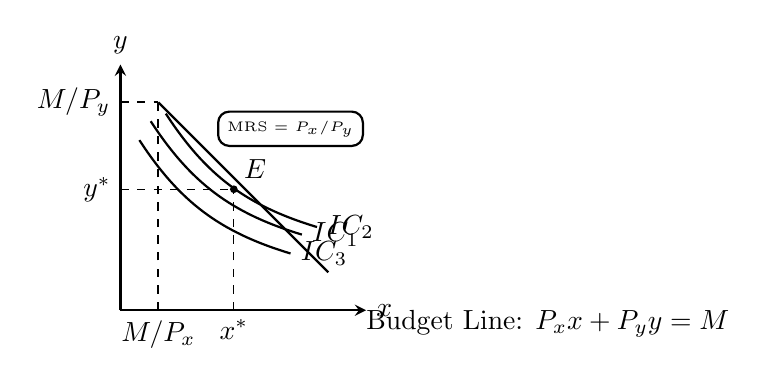
\begin{tikzpicture}[scale=0.48, thick, >=stealth]
    \draw[->] (0,0) -- (6.5,0) node[right] {$x$};
    \draw[->] (0,0) -- (0,6.5) node[above] {$y$};
    % Budget Line
    \draw[thick] (1,5.5) -- (5.5,1) node[below right=10pt] {Budget Line: $P_x x + P_y y = M$};
    \draw[dashed] (1,0) node[below] {$M/P_x$} -- (1,5.5);
    \draw[dashed] (0,5.5) node[left] {$M/P_y$} -- (1,5.5);
    % Indifference curves
    \draw[thick] (0.8,5) to[bend right=20] (4.8,2) node[right] {$IC_1$};
    \draw[thick] (1.2,5.2) to[bend right=20] (5.2,2.2) node[right] {$IC_2$};
    \draw[thick] (0.5,4.5) to[bend right=20] (4.5,1.5) node[right] {$IC_3$};
    % Equilibrium point E
    \filldraw (3,3.2) circle (2pt) node[above right] {$E$};
    \draw[dashed, thin] (3,0) node[below] {$x^*$} -- (3,3.2);
    \draw[dashed, thin] (0,3.2) node[left] {$y^*$} -- (3,3.2);
    \node[draw, fill=white, rounded corners, font=\tiny] at (4.5,4.8) {MRS = $P_x/P_y$};
\end{tikzpicture}
\end{center}
\textit{At $E$, the budget line is tangent to the highest attainable indifference curve ($IC_2$). $IC_3$ is unattainable; $IC_1$ is suboptimal. $MRS = P_x/P_y$.}

\subsection*{Consumer Equilibrium: Corner Solution}
\begin{center}
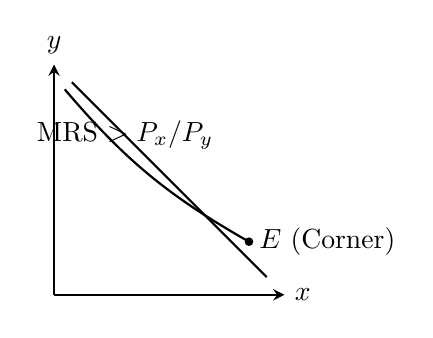
\begin{tikzpicture}[scale=0.45, thick, >=stealth]
    \draw[->] (0,0) -- (6.5,0) node[right] {$x$};
    \draw[->] (0,0) -- (0,6.5) node[above] {$y$};
    \draw (0.5,6) -- (6,0.5);
    \draw[thick] (0.3,5.8) to[bend right=10] (5.5,1.5);
    \filldraw (5.5,1.5) circle (2.5pt) node[right] {$E$ (Corner)};
    \node at (2,4.5) {MRS $> P_x/P_y$};
\end{tikzpicture}
\end{center}
\textit{Corner solution: Consumer spends all income on $x$ because $MU_x/P_x > MU_y/P_y$ everywhere, including at $y=0$. Indifference curve is flatter than budget line at the boundary.}

\subsection*{Income Consumption Curve (ICC) -- Normal Goods}
\begin{center}
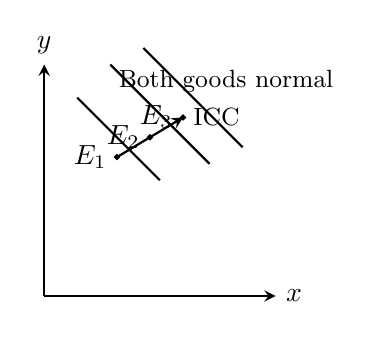
\begin{tikzpicture}[scale=0.42, thick, >=stealth]
    \draw[->] (0,0) -- (7,0) node[right] {$x$};
    \draw[->] (0,0) -- (0,7) node[above] {$y$};
    \draw (1,6) -- (3.5,3.5); \draw (2,7) -- (5,4);
    \draw (3,7.5) -- (6,4.5);
    \filldraw (2.2,4.2) circle (1.5pt) node[left] {$E_1$};
    \filldraw (3.2,4.8) circle (1.5pt) node[left] {$E_2$};
    \filldraw (4.2,5.4) circle (1.5pt) node[left] {$E_3$};
    \draw[thick, ->] (2.2,4.2) -- (3.2,4.8) -- (4.2,5.4) node[right] {\small ICC};
    \node at (5.5,6.5) {\small Both goods normal};
\end{tikzpicture}
\end{center}
\textit{ICC traces equilibrium points as income rises. Upward sloping $\to$ both goods are normal.}

\subsection*{Price Consumption Curve (PCC) and Derivation of Demand}
\begin{center}
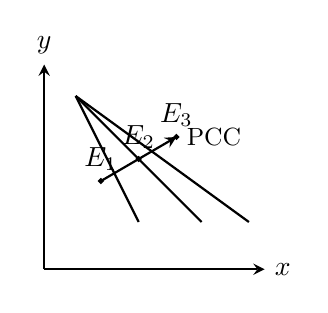
\begin{tikzpicture}[scale=0.4, thick, >=stealth]
    \draw[->] (0,0) -- (7,0) node[right] {$x$};
    \draw[->] (0,0) -- (0,6.5) node[above] {$y$};
    \draw (1,5.5) -- (3,1.5); \draw (1,5.5) -- (5,1.5);
    \draw (1,5.5) -- (6.5,1.5);
    \filldraw (1.8,2.8) circle (1.5pt) node[above] {$E_1$};
    \filldraw (3,3.5) circle (1.5pt) node[above] {$E_2$};
    \filldraw (4.2,4.2) circle (1.5pt) node[above] {$E_3$};
    \draw[thick, ->] (1.8,2.8) -- (3,3.5) -- (4.2,4.2) node[right] {\small PCC};
\end{tikzpicture}
\end{center}
\textit{PCC (or Offer Curve) traces equilibria as $P_x$ falls. From PCC, by plotting $P_x$ against $x^*$, we derive the Marshallian demand curve for $x$.}

\columnbreak

% ============================================================================
% PART 6: EFFECTS OF INCOME AND PRICE CHANGES
% ============================================================================
\section*{6. Income and Price Change Effects}

\subsection*{Income Effect (Income Change)}
When consumer's money income $M$ increases (prices constant), the budget line shifts \textbf{outward parallelly}. The new equilibrium occurs on a higher IC. The line joining equilibria at different income levels is the \textbf{Income Consumption Curve (ICC)}. From ICC, we derive the \textbf{Engel Curve}, showing relationship between income and quantity consumed.

\textbf{Classification by Good Type:}
\begin{itemize}[leftmargin=*,nosep]
    \item \textbf{Normal Good:} ICC slopes upward (both $x$ and $y$ rise with income). Engel curve has positive slope.
    \item \textbf{Inferior Good:} ICC bends backward (consumption of the inferior good falls as income rises, while the other good increases). Engel curve has negative slope beyond a certain income.
    \item \textbf{Luxury Good:} Consumption rises more than proportionately to income.
    \item \textbf{Necessity:} Consumption rises less than proportionately to income.
\end{itemize}

\subsection*{Price Effect (Price Change)}
When $P_x$ falls ($P_y$ and $M$ constant), the budget line \textbf{rotates outward} around the $y$-intercept. The $y$-intercept ($M/P_y$) remains unchanged; the $x$-intercept ($M/P_x$) increases. The line joining equilibria at different prices of $x$ is the \textbf{Price Consumption Curve (PCC)}.

\textbf{Total Price Effect Decomposition (Hicksian Method):}
For a fall in $P_x$:
\begin{enumerate}[leftmargin=*,nosep]
    \item \textbf{Total Effect (TE):} Movement from original equilibrium $E_1$ to final equilibrium $E_2$. $\Delta x = x_2 - x_1$.
    \item \textbf{Substitution Effect (SE):} Draw a hypothetical budget line parallel to the new budget line but tangent to the \textit{original indifference curve}. This removes the income effect (compensated). Movement from $E_1$ to $E_c$ (compensated point). $SE = x_c - x_1$. \textbf{Always positive} (for a price fall, consumption of the cheaper good rises).
    \item \textbf{Income Effect (IE):} Movement from $E_c$ to $E_2$. $IE = x_2 - x_c$. Sign depends on whether the good is normal (positive IE) or inferior (negative IE).
\end{enumerate}
\[
TE = SE + IE \quad \Rightarrow \quad \Delta x = \Delta x^s + \Delta x^i
\]

\subsection*{Graphical Decomposition for Normal Good ($P_x \downarrow$)}
\begin{center}
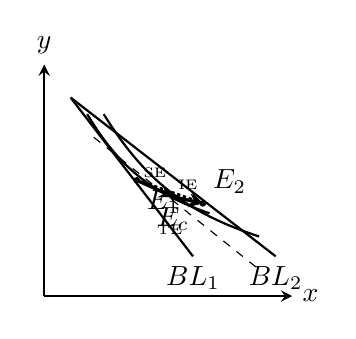
\begin{tikzpicture}[scale=0.42, thick, >=stealth]
    \draw[->] (0,0) -- (7.5,0) node[right] {$x$};
    \draw[->] (0,0) -- (0,7) node[above] {$y$};
    % Original BL
    \draw (0.8,6) -- (4.5,1.2) node[below] {$BL_1$};
    % New BL (Px fell)
    \draw (0.8,6) -- (7,1.2) node[below] {$BL_2$};
    % Hypothetical compensated BL
    \draw[dashed, thin] (1.5,4.8) -- (6.5,0.8);
    % ICs (bowed toward origin)
    \draw (1.3,5.5) to[bend right=20] (5,2.5); % IC1
    \draw (1.8,5.5) to[bend right=20] (6.5,1.8); % IC2
    % Points
    \filldraw (2.8,3.5) circle (1.8pt) node[below right] {$E_1$};
    \filldraw (4.8,2.8) circle (1.8pt) node[above right] {$E_2$};
    \filldraw (3.9,3) circle (1.8pt) node[below] {$E_c$};
    % Arrows
    \draw[->, very thick] (2.8,3.5) -- (3.9,3) node[midway, above] {\tiny SE};
    \draw[->, very thick] (3.9,3) -- (4.8,2.8) node[midway, above] {\tiny IE};
    \draw[->, very thick, densely dotted] (2.8,3.5) -- (4.8,2.8) node[midway, below=8pt] {\tiny TE};
\end{tikzpicture}
\end{center}
\textit{$TE = SE + IE$. For a normal good, both SE and IE work in same direction.}

\subsection*{Special Cases}
\begin{itemize}[leftmargin=*,nosep]
    \item \textbf{Inferior Good ($P_x \downarrow$):} SE positive (increase $x$), IE negative (decrease $x$, because income effect makes consumer feel richer and buy less of inferior good). TE sign ambiguous: if $|SE| > |IE|$, net demand rises (normal demand); if $|IE| > |SE|$, \textbf{Giffen good}, demand falls.
    \item \textbf{Perfect Substitutes:} Straight-line ICs. MRS constant. Equilibrium typically at a corner (consume only cheaper good). No interior tangency unless slopes are equal.
    \item \textbf{Perfect Complements:} L-shaped ICs. MRS not defined at the kink. Consumer always consumes goods in fixed proportions. Income expansion path is a ray from origin. Price change yields only an income effect (no substitution effect, because goods must be consumed together).
\end{itemize}

% ============================================================================
% PART 7: COMPARISON WITH MARSHALLIAN ANALYSIS
% ============================================================================
\section*{7. Indifference Curve vs. Marshallian Utility Analysis}

\begin{center}
\begin{tabular}{@{}p{2.8cm}p{2.8cm}@{}}
\toprule
\textbf{Marshallian (Cardinal)} & \textbf{Hicks-Allen (Ordinal)} \\
\midrule
Utility measurable in utils & Utility only ranked (ordinal) \\
Assumes constant MU of money & No such assumption \\
Law of Diminishing MU & Diminishing MRS (weaker) \\
Single-good analysis focus & Two-good (or multi-good) \\
Cannot separate IE and SE & Explicitly decomposes IE \& SE \\
Budget constraint implicit & Budget line explicit \\
Demand derived from MU = Price & Demand derived from MRS = Price Ratio \\
Substitution effect not isolated & Substitution effect via compensated budget \\
\bottomrule
\end{tabular}
\end{center}

\textbf{Advantage of Indifference Curve:} More general, fewer restrictive assumptions, better analytical tool for welfare, taxation, and policy analysis. The ordinal approach underpins all modern microeconomic consumer theory.

% ============================================================================
% PART 8: EXTENSIVE CASE STUDIES
% ============================================================================
\section*{8. Comprehensive Case Studies}

\subsection*{Case Study 1: Cash vs. In-Kind Transfers -- The Food Stamp Program (US SNAP)}

\textbf{Background:} Governments provide assistance to low-income households either through \textbf{cash transfers} (direct money) or \textbf{in-kind transfers} (specific goods like food stamps, housing vouchers). The US Supplemental Nutrition Assistance Program (SNAP, formerly Food Stamps) provides vouchers that can only be spent on food. Economists have long debated whether cash would be superior using indifference curve analysis.

\textbf{The Economic Question:} Given a fixed government expenditure, which type of transfer provides greater consumer satisfaction (higher utility)?

\textbf{Indifference Curve Analysis Setup:}
Two goods: \textbf{Food (F)} on x-axis, \textbf{All Other Goods (AOG)} on y-axis.

\textit{Initial Situation (No Transfer):} Budget line $BL_0$ with intercepts $M/P_F$ and $M/P_{AOG}$. Equilibrium at $E_0$ on $IC_0$.

\textit{Cash Transfer of Amount \$T:} Income increases by \$T. Budget line shifts outward parallelly from $BL_0$ to $BL_{\text{cash}}$. New equilibrium $E_{\text{cash}}$ on $IC_{\text{cash}}$.

\textit{In-Kind Transfer (Food Stamps of Value \$T, usable only for Food):} The budget line shifts rightward only for food. It becomes \textbf{kinked}: For food quantities up to \$T/$P_F$, the consumer can get them using stamps without sacrificing AOG (the budget line is horizontal at $y = M/P_{AOG}$ for $F \leq \text{stamp quantity}$). Beyond that, the budget line slopes down as usual.

\begin{center}
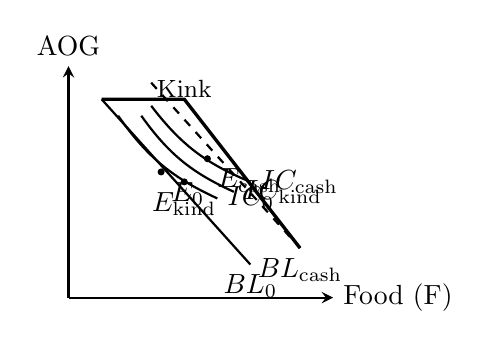
\begin{tikzpicture}[scale=0.42, thick, >=stealth]
    \draw[->] (0,0) -- (8,0) node[right] {Food (F)};
    \draw[->] (0,0) -- (0,7) node[above] {AOG};
    % Original BL
    \draw (1,6) -- (5.5,1) node[below] {$BL_0$};
    % Cash BL
    \draw[dashed] (2.5,6.5) -- (7,1.5) node[below] {$BL_{\text{cash}}$};
    % In-kind kinked BL
    \draw[very thick] (1,6) -- (3.5,6) -- (7,1.5);
    \node at (3.5,6.3) {\small Kink};
    % ICs
    \draw (1.5,5.5) to[bend right=15] (4.5,3) node[right] {$IC_0$};
    \draw (2.5,5.8) to[bend right=15] (5.5,3.5) node[right] {$IC_{\text{cash}}$};
    \draw (2.2,5.5) to[bend right=15] (5,3.2) node[right] {$IC_{\text{kind}}$};
    % Equilibrium points
    \filldraw (2.8,3.8) circle (2pt) node[below right] {$E_0$};
    \filldraw (4.2,4.2) circle (2pt) node[below right] {$E_{\text{cash}}$};
    \filldraw (3.5,3.5) circle (2pt) node[below] {$E_{\text{kind}}$};
\end{tikzpicture}
\end{center}

\textbf{Analysis of Outcomes:}

\textbf{Case A: Consumer Initially Buys Less Food Than Stamp Value.}
The consumer's optimal choice with stamps is at the kink (or beyond where the cash-equivalent BL is available). The in-kind transfer forces the consumer to a point on a \textbf{lower indifference curve} ($IC_{\text{kind}}$) than with cash ($IC_{\text{cash}}$). The consumer would prefer cash because they could allocate spending to more valued AOG rather than being forced to over-consume food relative to their preferences. \textbf{Cash is Pareto-superior} -- it gives the consumer the option to choose the same bundle as with stamps, but also others that yield higher utility.

\textbf{Case B: Consumer Initially Buys More Food Than Stamp Value.}
If the consumer already consumed more food than the stamp quantity, the in-kind transfer is \textbf{equivalent to cash} (the extra stamps simply free up money that would have been spent on food, which is then spent on AOG). The consumer reaches the same $IC_{\text{cash}}$. In this case, the restriction is non-binding.

\textbf{Empirical Evidence and Policy Implications:}
\begin{itemize}[leftmargin=*,nosep]
    \item Studies show most SNAP recipients are \textbf{infra-marginal} (Case B: their food spending exceeds the voucher amount), so the distortion is small for them.
    \item However, \textbf{marginal recipients} (new entrants, those with higher AOG preferences) would indeed be better off with cash.
    \item \textbf{Paternalism:} Policymakers often prefer in-kind transfers to ensure the money is spent on ``merit goods'' (food, housing, education) rather than ``temptation goods'' (alcohol, tobacco). This is a normative judgment overriding consumer sovereignty.
    \item \textbf{Political Economy:} Taxpayers may be more willing to fund food stamps than cash transfers, perceiving less ``waste.'' This political feasibility can make in-kind transfers more generous than cash, potentially making even recipients better off despite the distortion.
    \item The analysis demonstrates how indifference curves can evaluate \textbf{welfare effects of government policy} beyond simple cost analysis.
\end{itemize}

\textbf{Economic Lesson:} Indifference curve analysis provides a rigorous framework for comparing policy instruments. While cash is generally more efficient (higher utility per dollar spent), in-kind transfers may be justified on paternalistic or political grounds. The binding vs. non-binding constraint distinction is critical.

\subsection*{Case Study 2: Work-Leisure Choice and the Backward-Bending Labor Supply Curve}

\textbf{Background:} The labor supply decision involves a trade-off between two ``goods'': \textbf{Income} (consumption of goods) and \textbf{Leisure} (time not working). Indifference curve analysis explains why an increase in the wage rate may either increase or decrease hours worked, leading to a \textbf{backward-bending labor supply curve}.

\textbf{The Model:}
\begin{itemize}[leftmargin=*,nosep]
    \item \textbf{Goods on axes:} Leisure ($L$) on x-axis (hours per day), Income ($Y$) on y-axis.
    \item \textbf{Time Constraint:} $L + H = T$, where $H$ = hours worked, $T$ = total time endowment (e.g., 24 hours/day).
    \item \textbf{Budget Constraint:} $Y = w \cdot H = w (T - L)$. Slope $= -w$ (the wage rate is the opportunity cost of an hour of leisure).
    \item \textbf{Utility:} $U = U(Y, L)$. Leisure is a normal good (usually).
\end{itemize}

\textbf{Increase in Wage Rate ($w$): Decomposition.}
\begin{center}
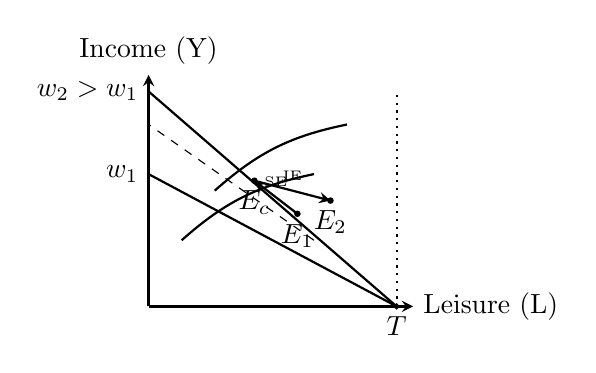
\begin{tikzpicture}[scale=0.42, thick, >=stealth]
    \draw[->] (0,0) -- (8,0) node[right] {Leisure (L)};
    \draw[->] (0,0) -- (0,7) node[above] {Income (Y)};
    % Time endowment
    \filldraw (7.5,0) circle (1.5pt) node[below] {$T$};
    \draw[dotted] (7.5,0) -- (7.5,6.5);
    % Budget lines
    \draw (7.5,0) -- (0,4) node[left] {$w_1$};
    \draw (7.5,0) -- (0,6.5) node[left] {$w_2 > w_1$};
    % Compensated BL (dashed)
    \draw[dashed, thin] (5,2) -- (0,5.5);
    % Indifference curves
    \draw (5,4) to[bend right=15] (1,2);
    \draw (6,5.5) to[bend right=15] (2,3.5);
    \filldraw (4.5,2.8) circle (1.8pt) node[below] {$E_1$};
    \filldraw (3.2,3.8) circle (1.8pt) node[below] {$E_c$};
    \filldraw (5.5,3.2) circle (1.8pt) node[below] {$E_2$};
    \draw[->] (4.5,2.8) -- (3.2,3.8) node[midway, above] {\tiny SE};
    \draw[->] (3.2,3.8) -- (5.5,3.2) node[midway, above] {\tiny IE};
\end{tikzpicture}
\end{center}

\textbf{Analysis:}
\begin{itemize}[leftmargin=*,nosep]
    \item \textbf{Substitution Effect (SE):} A higher wage makes leisure more expensive (higher opportunity cost). The consumer substitutes \textit{away} from leisure toward work (more income). $L \downarrow$, $H \uparrow$. SE is always positive for work.
    \item \textbf{Income Effect (IE):} A higher wage increases real income. If leisure is a \textbf{normal good}, the consumer ``buys'' more leisure (works less). $L \uparrow$, $H \downarrow$. IE is negative for work.
    \item \textbf{Net Effect:} Depends on relative magnitudes.
    \begin{itemize}[nosep]
        \item \textbf{At low wages:} SE dominates $\to$ wage increase $\to$ more work ($H \uparrow$). Labor supply curve slopes upward.
        \item \textbf{At high wages:} IE may dominate $\to$ wage increase $\to$ less work ($H \downarrow$). Labor supply curve bends backward.
    \end{itemize}
\end{itemize}

\textbf{Empirical Evidence:}
\begin{itemize}[leftmargin=*,nosep]
    \item Male labor supply is relatively inelastic; the backward bend is observed at very high income levels (e.g., professionals reducing hours, early retirement).
    \item Female labor supply elasticity is higher; participation decisions dominate.
    \item Over the 20th century, wages rose dramatically, yet average weekly hours fell (from 60+ to ~40), consistent with a dominant long-run income effect.
    \item Recent studies of ride-share drivers (Uber, Lyft) show strong evidence of income targeting behavior -- drivers work less when hourly earnings are high, indicating a strong income effect (reference-dependent preferences).
\end{itemize}

\textbf{Policy Implications:}
\begin{enumerate}[leftmargin=*,nosep]
    \item \textbf{Taxation and Labor Supply:} A tax cut raises the after-tax wage. Whether it increases labor supply depends on the relative strength of SE and IE. The Laffer curve concept depends partly on this.
    \item \textbf{Overtime Pay:} Premium overtime wages (1.5x, 2x) have both SE (more incentive to work extra hours) and IE (higher overall income), making the net effect on total hours ambiguous.
    \item \textbf{Welfare Programs:} Design of welfare/transfer programs (Earned Income Tax Credit -- EITC) must consider labor supply responses. EITC increases effective wages for low-income workers (SE dominant) while providing income support, encouraging work.
\end{enumerate}

\textbf{Economic Lesson:} The work-leisure model demonstrates the power of indifference curve analysis in decomposing complex behavioral responses to economic incentives, with profound implications for tax and welfare policy.

% ============================================================================
% PART 9: EXAM QUESTIONS
% ============================================================================
\section*{9. Exam Questions \& Model Answers}

\subsection*{Question 1: Properties and Proof}
\textbf{Prove that two indifference curves cannot intersect.}

\textbf{Answer:} Assume two indifference curves $IC_1$ and $IC_2$ intersect at point $A$. Since $A$ is on both curves, the consumer is indifferent between $A$ and any other point on $IC_1$, and also between $A$ and any point on $IC_2$. Choose point $B$ on $IC_1$ and point $C$ on $IC_2$ such that $C$ has more of both goods than $B$. Since $A$ is on $IC_1$, consumer is indifferent between $A$ and $B$. Since $A$ is on $IC_2$, consumer is indifferent between $A$ and $C$. By transitivity, consumer must be indifferent between $B$ and $C$. But $C$ has more of both goods than $B$; by non-satiation, $C$ is strictly preferred to $B$. Contradiction. Therefore, indifference curves cannot intersect.

\vspace{0.2cm}

\subsection*{Question 2: Equilibrium and Comparative Statics}
\textbf{A consumer has $U = x^{0.5} y^{0.5}$. $P_x = 2$, $P_y = 4$, $M = 120$.}
\textbf{(a) Find optimal bundle.}
\textbf{(b) If $P_x$ falls to \$1, find new equilibrium and decompose total effect using Hicksian method.}
\textbf{(c) Derive the demand function for $x$ and the equation of the Price Consumption Curve.}

\vspace{0.1cm}
\textbf{Solution:}
\textbf{(a)} $MU_x = 0.5 x^{-0.5} y^{0.5}$, $MU_y = 0.5 x^{0.5} y^{-0.5}$.
$MRS = MU_x/MU_y = y/x$. At equilibrium: $y/x = 2/4 = 1/2 \Rightarrow y = 0.5x$.
Budget: $2x + 4(0.5x) = 120 \Rightarrow 2x + 2x = 120 \Rightarrow 4x = 120 \Rightarrow \mathbf{x=30, y=15}$.

\textbf{(b)} New $P_x = 1$. MRS = $P_x/P_y \Rightarrow y/x = 1/4 \Rightarrow y = 0.25x$.
Budget: $1x + 4(0.25x) = 120 \Rightarrow x + x = 120 \Rightarrow 2x=120 \Rightarrow \mathbf{x=60, y=15}$.
\textit{Total Effect:} $\Delta x = 60 - 30 = +30$.

\textit{SE (Hicks):} Find utility at $E_1$: $U = 30^{0.5} \cdot 15^{0.5} = \sqrt{450} \approx 21.21$. Find bundle at new prices ($P_x=1, P_y=4$) that gives this $U$ at minimum cost: $y/x = 0.25 \Rightarrow y=0.25x$. $U = x^{0.5}(0.25x)^{0.5} = x^{0.5} \cdot 0.5 x^{0.5} = 0.5x = 21.21 \Rightarrow x_c = 42.42$.
$SE = 42.42 - 30 = +12.42$ (increase in $x$ due to relative price change only).
$IE = 60 - 42.42 = +17.58$ (increase in $x$ because real income rose).
Since $IE > 0$, $x$ is a normal good (and a luxury here since spending on $x$ remains constant at \$60).

\textbf{(c)} Demand for $x$ (from MRS condition $y/x = P_x/P_y \Rightarrow P_x x = P_y y$): Income is spent equally. $P_x x = M/2$. Demand: $\mathbf{x = M/(2P_x)}$. PCC equation: $y = (P_x/P_y) x$, but $P_x x = M/2$, so $y = M/(2P_y)$ constant. PCC is a \textbf{horizontal line} at $y = M/(2P_y)$ (both goods normal, and in Cobb-Douglas with equal exponents, expenditure on $y$ is fixed when $M$ constant but $P_x$ changes). More generally, the PCC is the locus of points satisfying $y/x = P_x/P_y$ with $P_x x + P_y y = M$ as $P_x$ varies. Here it simplifies.

\vspace{0.2cm}

\subsection*{Question 3: Conceptual}
\textbf{Using indifference curve analysis, explain why the demand curve for a normal good must slope downwards.}

\textbf{Answer:} Consider a fall in $P_x$:
\begin{itemize}[leftmargin=*,nosep]
    \item \textbf{Substitution Effect:} The relative price of $x$ falls. Holding real income constant, the consumer substitutes toward $x$ and away from $y$. $x$ increases. This effect is always negative (price falls $\to$ quantity rises).
    \item \textbf{Income Effect:} The price fall increases real income. For a \textbf{normal good}, higher real income leads to an increase in consumption. So $x$ increases further.
\end{itemize}
Both effects work in the same direction: $x$ unambiguously rises when $P_x$ falls. Therefore, the demand curve (plotting $P_x$ against $x$) must be \textbf{downward sloping}. There is no theoretical possibility of an upward-sloping demand curve for a normal good. The Giffen paradox can only arise for strongly inferior goods where the negative income effect (less $x$ as real income rises) outweighs the substitution effect.

\vspace{0.2cm}

\subsection*{Question 4: Application}
\textbf{A government subsidizes the price of a staple food for low-income households. Using indifference curve analysis, compare this price subsidy to an equivalent-value cash transfer. Which policy places the consumer on a higher indifference curve? Why might the government still choose the price subsidy?}

\textbf{Answer:} A price subsidy rotates the budget line outward specifically for the subsidized good (change in relative prices). A cash transfer shifts the budget line outward parallelly. For the same government cost, the cash transfer generally places the consumer on a \textbf{higher indifference curve} because it imposes no restriction on consumption choices (the consumer can always choose the same bundle as under the subsidy, but may prefer a different one). The price subsidy introduces a distortion: it artificially lowers the relative price, encouraging overconsumption of the subsidized good relative to the consumer's true preferences ($MRS \neq P_x/P_y$ at the equilibrium without further adjustment by the consumer).

\textbf{However}, governments may prefer price subsidies due to:
\begin{itemize}[nosep]
    \item \textbf{Paternalism:} Ensuring the good consumed is nutritious food rather than potentially harmful alternatives.
    \item \textbf{Externalities:} If consumption of the good has positive externalities (e.g., healthier children $\to$ lower public health costs), the price subsidy can correct an underconsumption problem.
    \item \textbf{Political acceptability:} Taxpayers may be more willing to fund food subsidies than unrestricted cash.
    \item \textbf{Intra-household allocation:} Cash may be captured by certain household members and not benefit children; in-kind transfers may target intended beneficiaries better.
\end{itemize}

\end{multicols}

% ============================================================================
% SUMMARY TABLE
% ============================================================================
\vspace{0.3cm}
\begin{center}
\fbox{\begin{minipage}{0.9\textwidth}
\footnotesize
\textbf{Summary Cheat Sheet: Indifference Curve Analysis}
\begin{center}
\begin{tabular}{@{}p{3.2cm}p{2.8cm}p{3.2cm}@{}}
\toprule
\textbf{Concept} & \textbf{Key Formula/Condition} & \textbf{Significance} \\
\midrule
Indifference Curve & $U(x,y) = \text{const}$ & Bundles yielding equal satisfaction \\
MRS & $MU_x / MU_y$ & Slope of IC; willingness to trade \\
Budget Line & $P_x x + P_y y = M$ & Affordable bundles; slope $= -P_x/P_y$ \\
Consumer Equilibrium & $MRS = P_x/P_y$ & Tangency of IC and BL \\
Income Consumption Curve & Locus of equilibria as $M$ varies & Basis for Engel curve \\
Price Consumption Curve & Locus of equilibria as $P_x$ varies & Basis for demand curve \\
Substitution Effect & Movement along original IC to new price ratio & Always non-positive for own price \\
Income Effect & Movement to new IC (shift) & Sign depends on good type \\
Total Effect & $TE = SE + IE$ & Decomposes price effect \\
\bottomrule
\end{tabular}
\end{center}

\vspace{0.1cm}
\textbf{Quick Reference: Effects of $P_x \downarrow$}
\begin{itemize}[leftmargin=*,nosep]
    \item Normal Good: SE $+$ and IE $+$ $\to$ unambiguous $x \uparrow$, Demand slopes down.
    \item Inferior (non-Giffen): SE $+$, IE $-$ but $|SE| > |IE|$ $\to$ $x \uparrow$, Demand slopes down.
    \item Giffen Good: SE $+$, IE $-$ and $|IE| > |SE|$ $\to$ $x \downarrow$, Demand slopes up (rare).
\end{itemize}
\end{minipage}}
\end{center}

\end{document}